\documentclass{article}
\usepackage[utf8]{inputenc}

% used for figures
\usepackage{graphicx}
\usepackage{placeins} 

% used for plotting math
\usepackage{amsmath}
\usepackage{breqn}
\usepackage{mathdots}

% used for writing code
\usepackage{pythonhighlight}
\renewcommand{\lstlistingname}{Algorithme}

% used for bibliography
\usepackage{hyperref}
\usepackage{apacite}[natbibapa]
\usepackage[english]{babel}
\addto{\captionsenglish}{%
    \renewcommand{\refname}{Références}}

% titles
\title{Titre}
\author{Alexi Morin}
\date{Mois 2021}

% doesn't work
\DeclareUnicodeCharacter{2212}{-}

% used to write the bibliography in the same file
\begin{filecontents*}[overwrite]{references.bib}
@article{sneddon1946distribution,
  title={The distribution of stress in the neighbourhood of a crack in an elastic solid},
  author={Sneddon, Ian Naismith},
  journal={Proceedings of the Royal Society of London. Series A. Mathematical and Physical Sciences},
  volume={187},
  number={1009},
  pages={229--260},
  year={1946},
  publisher={The Royal Society London}
}
@article{lecampion2022geomechanics,
  title={Computational geomechanics: Course notes},
  author={Lecampion, Brice},
  year={2022},
  publisher={École Polytechnique Fédérale de Lausanne}
}
\end{filecontents*}


\begin{document}

% introduction page starts here
\begin{titlepage}
    \begin{center}
        \vspace*{1cm}
         \Huge  
        Computational geomechanics
         \vspace{0.5cm}
        \textbf{Evolution of a pressurized fracture}
         \vspace{0.5cm}
        \\ 
            
        \vspace{1.5cm}
            
        Alexi Morin
            
        \vfill
            
	Report presented to\\
	Prof. Brice Lecampion
  
        \vspace{2.cm}
            

        \Large

        Department of Civil Engineering\\
        École Polytechnique Fédérale de Lausanne\\
        Lausanne, Vaud, Switzerland\\
        Fall 2022
            
    \end{center}
\end{titlepage}

% do not change the different sections

\section{Problem introduction}
We are interested in the evolution of a pressurized fracture in rock. A typical configuration of this problem would involve a wellbore in which a fluid is injected with the goal of causing the propagation of fractures in the medium (figure \ref{fig:conceptual}). 

\begin{figure}[h]
    \centering
    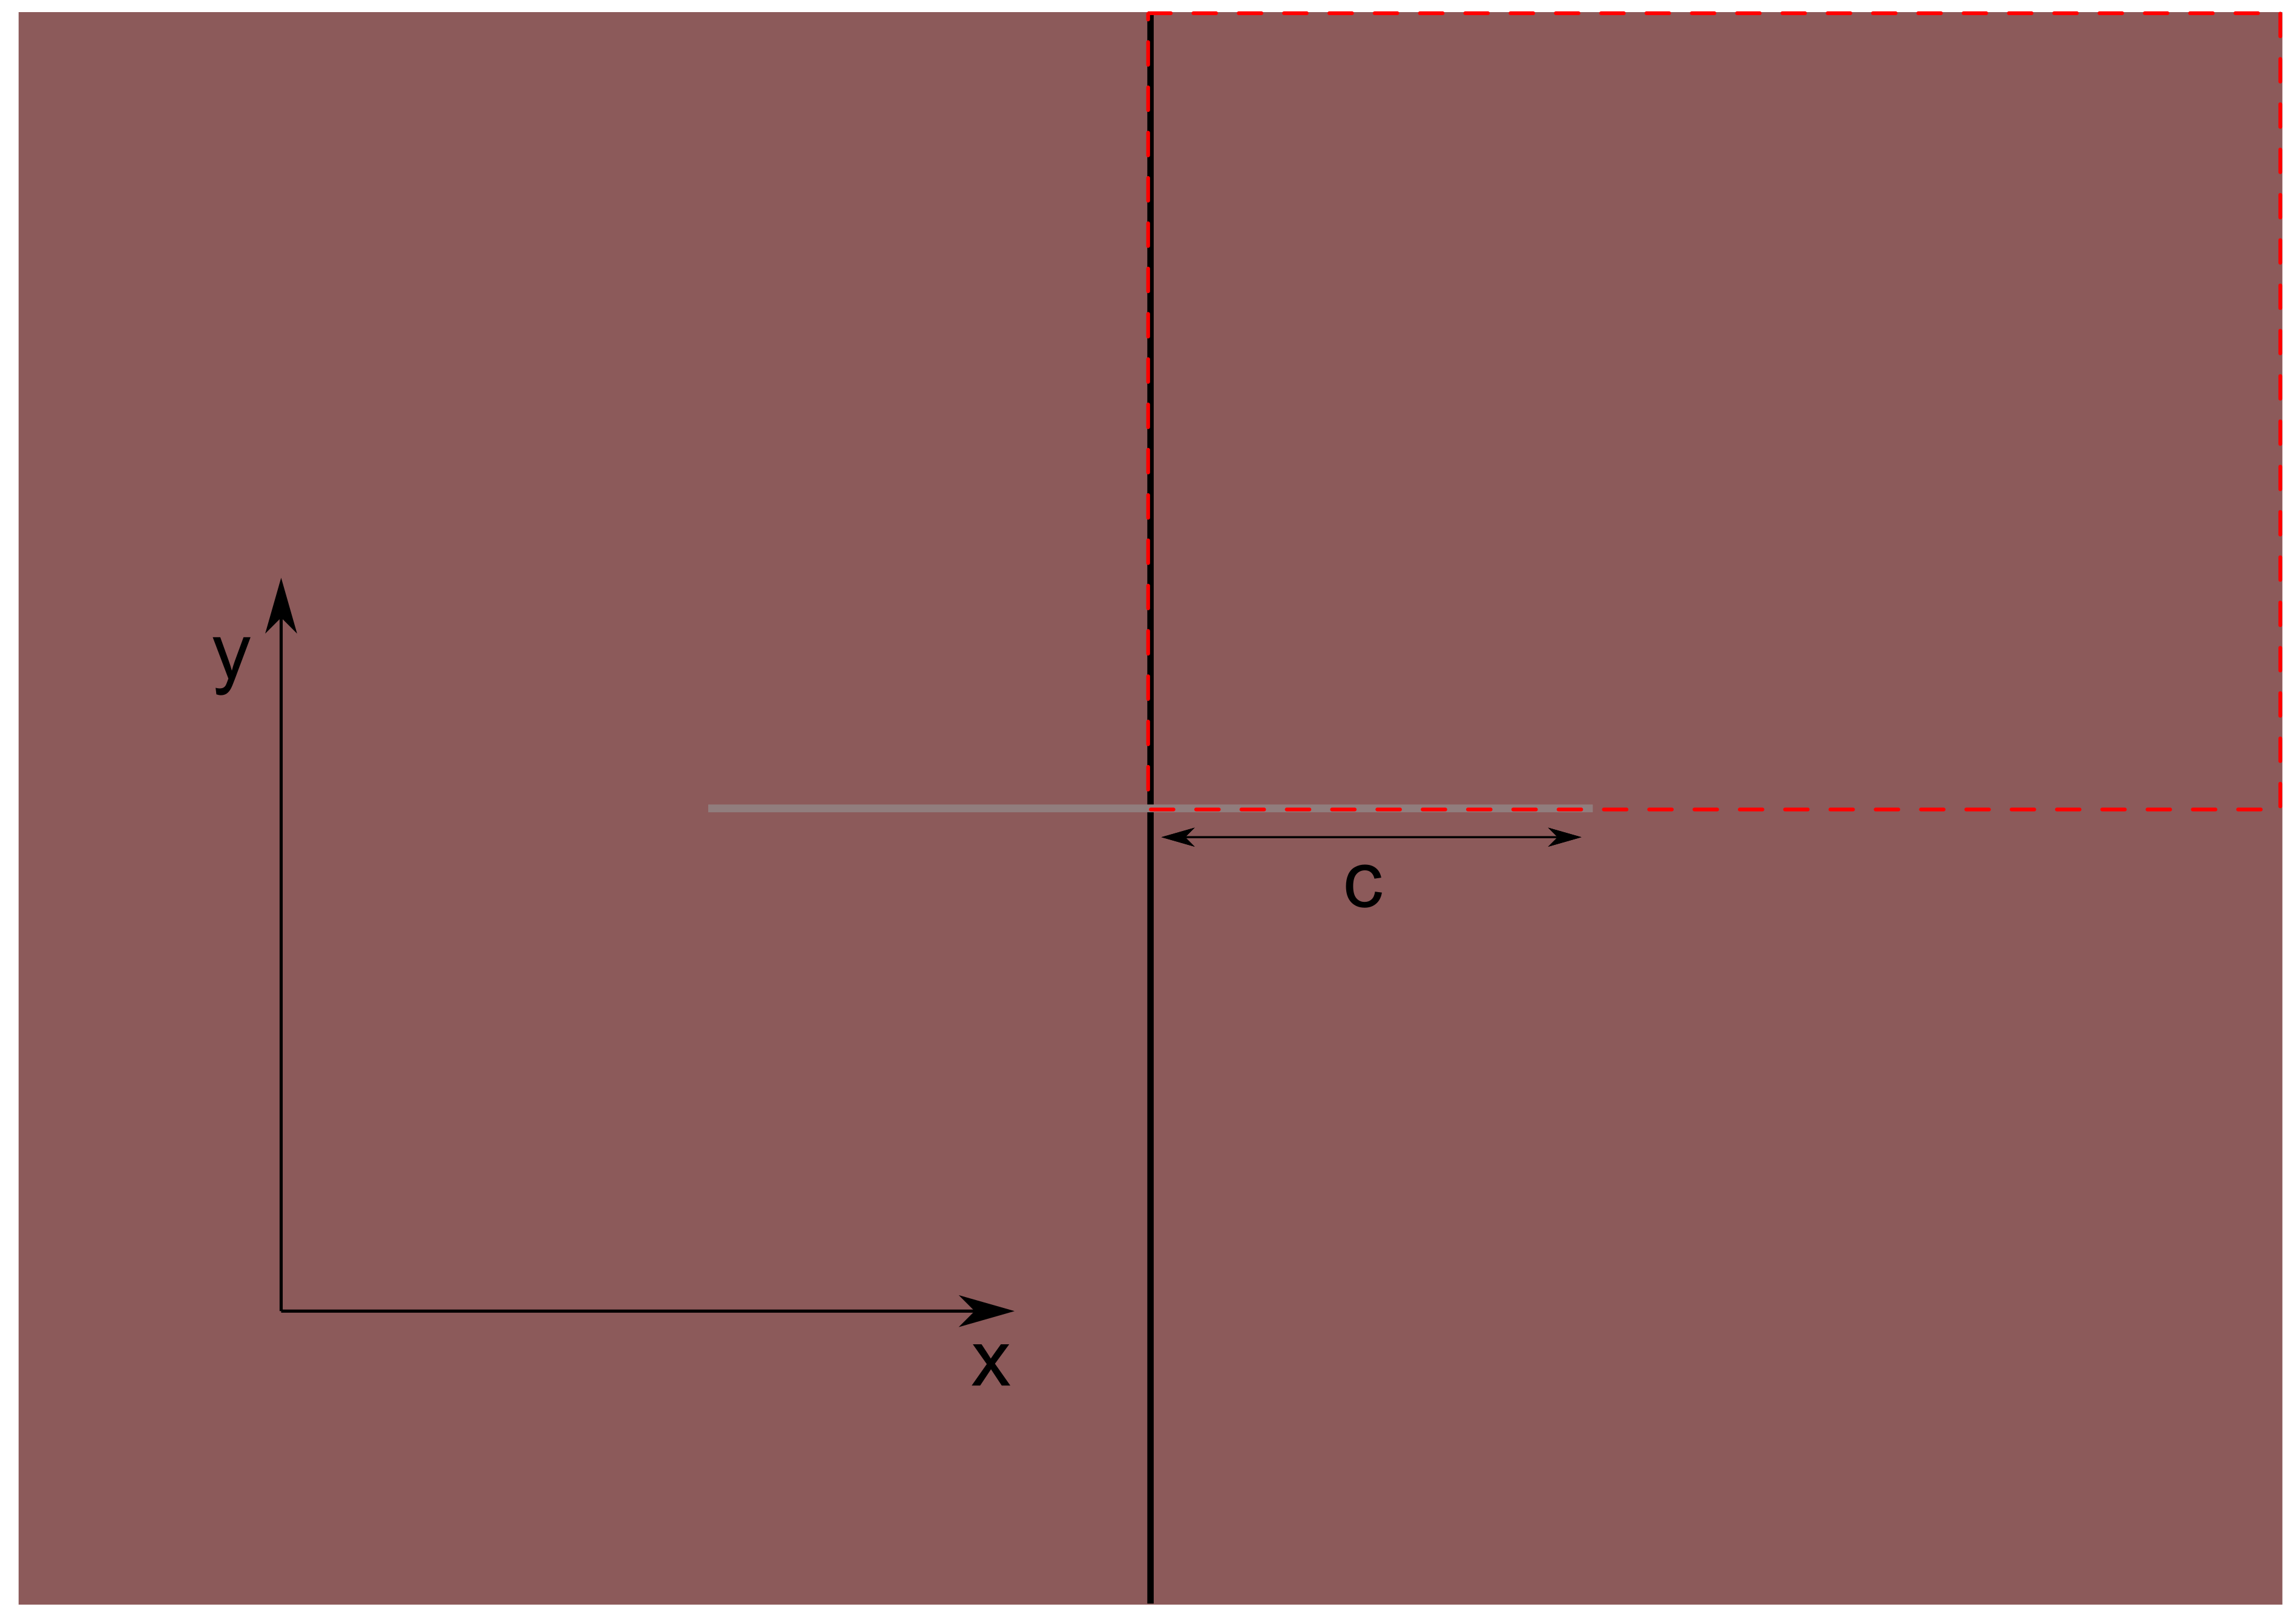
\includegraphics[width=0.75\textwidth]{fracture}
    \caption{Conceptual model of the problem. The region highlighted by the red dashed line shows the modeled domain, simplified by the symmetry of the problem.}
    \label{fig:conceptual}
\end{figure}

In reality, this medium would be anisotropic and heterogeneous, for the fracturation is typically done in layered sedimentary rocks. We will however use the following simplifying assumptions to model this scenario with finite elements:

\begin{itemize}
	\item The rock will be considered homogeneous and isotropic. This is not an implementation complexity but will greatly facilitate the analysis of the results.
	\item The fracture will be considered planar, of finite length $c$ in one direction and of infinite length in the other. This will greatly simplify the implementation as we won't deal with the non-linearities related to plasticity and fracture propagation. This will also let us reduce the modeled domain because of the symmetry (see figure \ref{fig:conceptual}).
	\item The pressure at the fracture will be directly applied as a boundary condition. A boundary condition closer to reality would be to apply a known flux i.e. the fluid injection rate. However, this would imply the need for a fluid flow law in fractured medium, further complexifying the implementation.
\end{itemize}
%
With these assumptions set, we will be interested in investigating both the undrained and drained response of the fracture to the applied pressure, tracking it's deformation and surrounding stress through time. We will be able to compare the results to an analytical solution from \citeA{sneddon1946distribution}. Finally, we will face two ways of applying pressure to the crack:


\begin{itemize}
	\item An impermeable fracture scenario, where only a mechanical pressure $\sigma_{\text{frac}}$ is applied in the vertical direction.
	\item A permeable fracture scenario, where both a mechanical pressure $\sigma_{\text{frac}}$ and a fluid pressure $p_{\text{frac}}$ are applied. Note that $\sigma_{\text{frac}} = p_{\text{frac}}$.
\end{itemize}
%
With those two scenarios, we will compare the amount of fluid flow injected in the medium.

\section{Methodology}

In order to properly model the problem presented earlier, we need to properly define the boundary conditions, the geomechanical properties and, of course, the mathematical expressions needed to model poroelasticity using finite elements.

\subsection{Poroelasticity and finite element modelling}

A matrix form equation representing linear poroelasticity would be

\begin{equation}
	\begin{bmatrix}
	\mathbf{0} & \mathbf{0} \\
	\mathbf{0} & \mathbf{C} \\
	\end{bmatrix}
	\begin{pmatrix}
	\mathbf{u} \\
	\mathbf{p} \\
	\end{pmatrix}
+
	\begin{bmatrix}
	\mathbf{K} & \mathbf{-A} \\
	\mathbf{-A^T} & \mathbf{-S} \\
	\end{bmatrix}
	\begin{pmatrix}
	\dot{\mathbf{u}} \\
	\dot{\mathbf{p}} \\
	\end{pmatrix}
=
	\begin{pmatrix}
	\dot{\mathbf{f}_t} \\
	{\mathbf{f}_q} \\
	\end{pmatrix},
	\label{eq:fem}
\end{equation}
where $\mathbf{K}$ is the stiffness matrix, scaling with Young's modulus $\mathrm{E}$ and Poisson's ratio $\nu$, $\mathbf{S}$ is the storage matrix, scaling inversely with Biot's modulus $\mathrm{M}$, $\mathbf{C}$ is the conductivity matrix, scaling with the hydraulic conductivity $\mathrm{K}$, and finally $\mathbf{A}$ is the coupling matrix, linking elasticity and fluid flow with $\alpha$, Biot's coefficient \cite{lecampion2022geomechanics}. Using $\dot{\mathbf{x}}$ to denote the temporal rate of change of $\mathbf{x}$, we have $\mathbf{u}$ and $\mathbf{p}$ being the displacements and pressure, $\dot{\mathbf{f}_t}$ and ${\mathbf{f}_q}$ being the force vectors related to stress and fluid pressure (or flux) respectively. We will use an implicit Euler scheme, unconditionally stable and first order accurate in time. We can then re-write equation \ref{eq:fem} to
\begin{equation}
\begin{bmatrix}
\mathbf{K} & \mathbf{-A} \\
\mathbf{-A^T} & \mathbf{-S} - \Delta t\mathbf{C}  \\
\end{bmatrix}
\begin{pmatrix}
\Delta\mathbf{u}^n \\
\Delta\mathbf{p}^n \\
\end{pmatrix}
=
\Delta t
\begin{pmatrix}
\dot{\mathbf{f}_t} \\
\mathbf{f}_q \\
\end{pmatrix}
-
\begin{bmatrix}
\mathbf{0} & \mathbf{0} \\
\mathbf{0} & -\Delta t\mathbf{C} \\
\end{bmatrix}
\begin{pmatrix}
\mathbf{u}^n \\
\mathbf{p}^n \\
\end{pmatrix}.
\end{equation}
We can synthesize this to a simple linear system of equation, meaning that we can we find the update vector 
$\begin{pmatrix}
\Delta\mathbf{u}^n \\
\Delta\mathbf{p}^n \\
\end{pmatrix}$
by solving 
\begin{equation}
\mathbf{T}
\begin{pmatrix}
\Delta\mathbf{u}^n \\
\Delta\mathbf{p}^n \\
\end{pmatrix}
=
\mathbf{f_{\text{tot}}},
\end{equation}
used to find the displacements and pressure at time $t + \Delta t$ (or time step $n+1$) with
\begin{equation}
\begin{pmatrix}
\mathbf{u}^{n+1} \\
\mathbf{p}^{n+1} \\
\end{pmatrix}
=
\begin{pmatrix}
\mathbf{u}^{n} \\
\mathbf{p}^{n} \\
\end{pmatrix}
+
\begin{pmatrix}
\Delta\mathbf{u}^n \\
\Delta\mathbf{p}^n \\
\end{pmatrix}.
\end{equation}

\subsection{Domain, boundary conditions and mesh}
As described earlier, we can use the symmetry emerging from the hypothesis that the fracture is planar, of finite length $c$ in one direction and of infinite length in the other. This let us model the fracture in 2D plane strain, also restricting ourselves to a quarter of the domain (figure \ref{fig:domain}). 
%
\begin{figure}[h]
    \centering
    \includegraphics[width=0.75\textwidth]{fracture_boundaries}
    \caption{Conceptual model of the problem. The region highlighted by the red dashed line shows the modeled domain, simplified by the symmetry of the problem. The lines perpendicular to the domain boundary show normal movement restriction, while the arrows show where a known stress is applied.}
    \label{fig:domain}
\end{figure}
%
This symmetry will force us to use typical symmetrical boundary conditions for the left and bottom boundaries, meaning that neither orthogonal displacement nor fluid flow are possible. To generate an initial stress field, we will impose an isotropic traction on the top and right boundaries $\sigma_0$. Finally, an initial homogeneous pressure $p_0$ will be imposed everywhere. To ensure simplicity and facilitate the analysis of the results, we will set the initial pressure and stress field to 0 MPa, i.e. $p_0=\sigma_0=0$ (meaning that computing the initial stress field is redundant, but is done anyway for generality). The most interesting boundary conditions are the ones related to the fracture. As was described earlier, we will model two scenarios, one where the fracture is impermeable and one where the fracture is permeable. In the first case, only a vertical mechanical pressure $\sigma_{frac}$ will be applied at the fracture location. This means that we will have to make vertical displacements at those nodes possible. In the second scenario, we will apply both a mechanical pressure $\sigma_{frac}$ and a constant fluid pressure $p_{frac}$. Finally, stresses will be highly singular at the tip of the fracture. We will then need a very fine mesh around location $(1c, 0)$ (figure \ref{fig:domain}). We will also use quadratic triangle elements to better model the phenomenon. In order to not have edge effects from the finite dimensions of the domain, we will model a region 20 times larger than the fracture length $c$.

\begin{figure}[h]
    \centering
    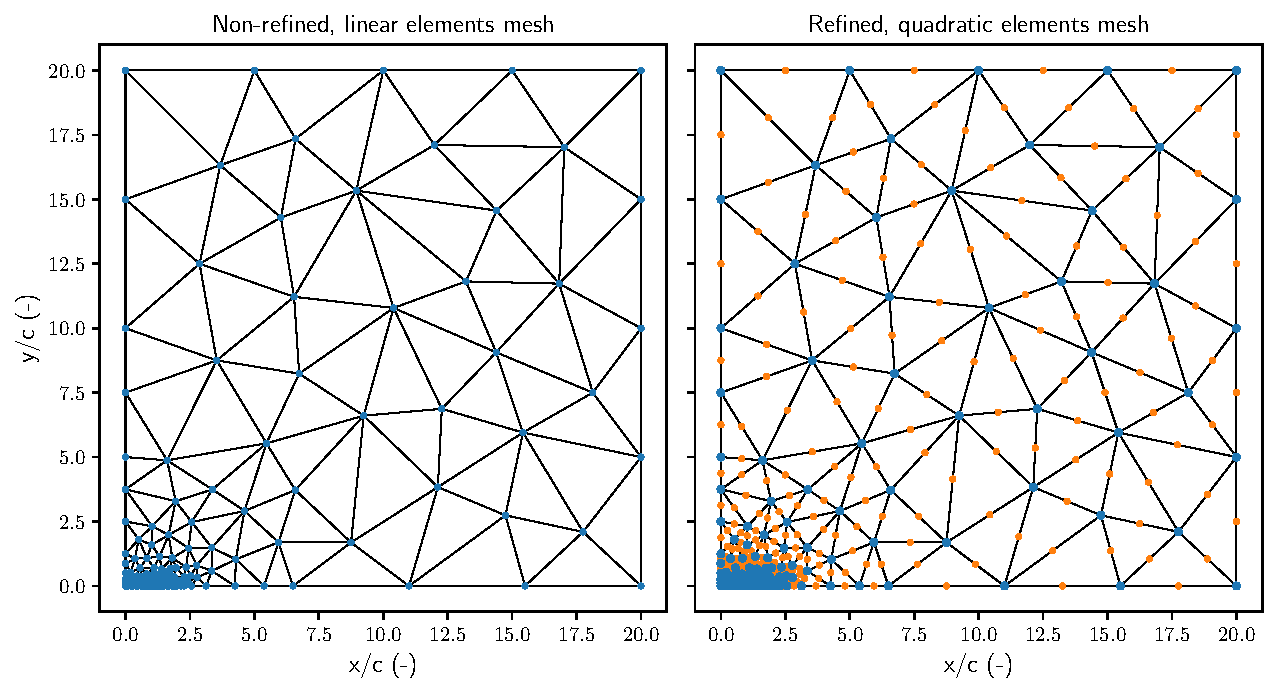
\includegraphics[width=1\textwidth]{../figures/mesh}
    \caption{The mesh used for the problem. While \textbf{a)} shows the whole domain, \textbf{b)} is zoomed in to highlight the finesse of the mesh near the fracture tip.}
    \label{fig:domain}
\end{figure}

\subsection{Geomechanical properties}

While the need to have realistic geomechanical properties is taken into account by proper dimensionality reduction, the undrained/drained behavior of the phenomenon makes it so that we cannot just set every physical parameter to unity. The table below highlights the physical parameters, their symbol and their values used in the model. The chosen values are meant to represent a Ohio sandstone and are taken from \citeA{lecampion2022geomechanics}.

\begin{table}[h]
\center
\begin{tabular}{|cccc|}
\hline 
Physical parameter & Symbol & Value & Unit \\ 
\hline \hline
Shear modulus & $\mathrm{G}$ & 6.8 & GPa \\ 
\hline 
Bulk modulus & $\mathcal{K}$ & 8.4 & GPa \\ 
\hline 
Biot's modulus & $\mathrm{M}$ & 9.18 & GPa \\ 
\hline 
Biot's coefficient & $\alpha$ & 0.71 & - \\ 
\hline 
Young's modulus & $\mathrm{E}$ & 16.07 & GPa \\ 
\hline 
Poisson's ratio & $\nu$ & 0.28 & - \\ 
\hline 
Undrained bulk modulus & $\mathcal{K}_u$ & 13.03 & GPa \\ 
\hline 
Undrained Young's modulus & $\mathrm{E}_u$ & 16.07 & GPa \\ 
\hline 
Undrained poisson's ratio & $\nu_u$ & 0.181 & - \\ 
\hline
Hydraulic conductivity & $\mathrm{K}$ & 1E-09 & m/s \\ 
\hline

\end{tabular} 
\caption{Geomechanical parameters}
\label{tab:params}
\end{table}
\FloatBarrier

\subsection{Dimensional reduction}

We can build normalization factors to try and generalize the results, independently of units. Following \citeA{sneddon1946distribution}, the fracture opening scales with
\begin{equation}
\epsilon = \frac{2c(1 - \sigma^2) \, p_{\text{frac}}}{\mathrm{E}} \dot{=} [\mathrm{L}].
\label{eq:eps}
\end{equation}
We can then normalize the resulting displacements $u_y$ by $\epsilon$, plotting the normalized displacements $u_y/\epsilon$ as a function of distance from crack length $c$, $x/c$. We also need to normalize the stresses. This is easily done by once again following \citeA{sneddon1946distribution}, where we can divide the computed stress by $p_{\text{frac}}$. Finally, the problem shows a temporal evolution component and we will need to normalize the results relative to this variable. The parameters related to the diffusion of fluid through the medium are the principal contributors controlling the the time-dependent behavior of the phenomenon. Since the hydraulic conductivity K has dimensions of $\mathrm{L}\,\mathrm{T}^{-1}$, we can normalize the time $t$ by multiplying it by a new coefficient
\begin{equation}
\theta = \frac{\mathrm{K}}{\epsilon} \dot{=} [\mathrm{T}^{-1}].
\end{equation}
\section{Results}

We can compare the results with the solution from \citeA{sneddon1946distribution}. The displacement $u_y$ of a fracture after a punch in a homogeneous medium reads

\begin{equation}
u_y = \epsilon\sqrt{1 - \left(\frac{x}{c}\right)^2}.
\end{equation}
For the undrained displacement, we can simply use the undrained values for Young's modulus $E$ and Poisson's ratio $\nu$. The same (reference) also provides an analytical solution for the stress field in the medium. (reference) defines a stress field $Z$, where $z=x+iy$:

\begin{equation}
Z = p_{\text{frac}}\left(\frac{z}{\sqrt{z^2 - c^2}} - 1 \right).
\end{equation}

With this stress field, we can easily compute the stress tensor and it's vertical component $\sigma_y$:

\begin{equation}
\sigma_y = Re Z + y Im Z',
\end{equation}
where $Z'$ is the complex conjugate of $Z$. For obtaining the stress at the crack, where $y=0$, the stress is simply the real component of $Z$. We can also show that $\sigma_x=\sigma_y$ at this boundary. We can now compare the displacements and the stress field at the fracture with our numerical solutions. It is interesting to note that the stress field is independent of both the geomechanical properties and time.

\subsection{Undrained displacements}

The computed undrained displacements for the analytical, impermeable and permeable numerical solutions (figure \ref{fig:undrained}a) are all very similar, also when compared with the relative error (figure \ref{fig:undrained}c). The relative error is greater in magnitude close to the fracture tip because of the analytical solution tending to zero. However, the stresses (figure \ref{fig:undrained}b) are different from the analytical solution from the permeable case at the fracture location. We can see an offset of around 1 times the pressure at the fracture $p_{\text{frac}}$. This is caused by the fact that the effective stress is different than in the impermeable case, of greater magnitude by exactly $1p_{\text{frac}}$. The relative error at this location is then close to 100\%. Since the stresses computed from the analytical solution are infinite at the fracture tip, we find the biggest errors at this location.

\begin{figure}[h]
    \centering
    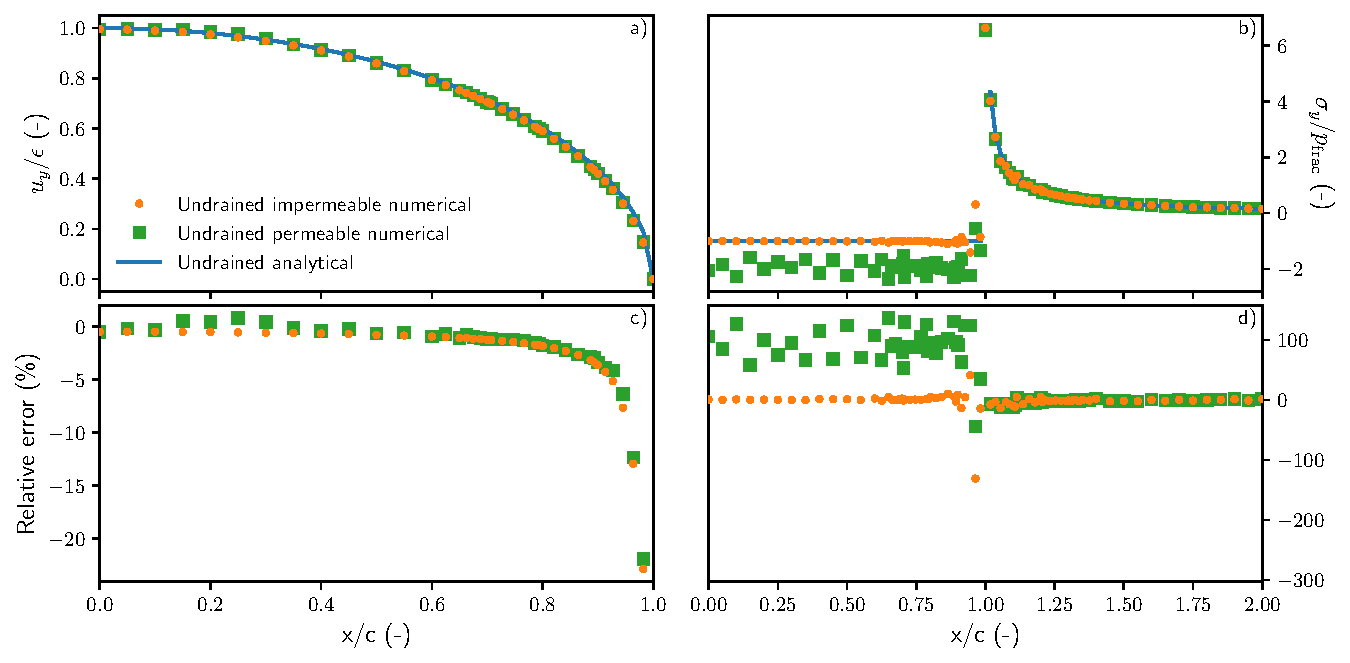
\includegraphics[width=1\textwidth]{../figures/undrained}
    \caption{Comparison of the displacements and stress for the undrained solution with the analytical solution for the cases of an impermeable and a permeable fracture. \textbf{a)} and \textbf{b)} compares the displacements and stress respectively, while \textbf{c)} and \textbf{d)} shows the relative error of the numerical solution for the displacement and stress.}
    \label{fig:undrained}
\end{figure}
\FloatBarrier

\subsection{Drained displacements}

The computed drained displacements for the analytical, impermeable and permeable numerical solutions (figure \ref{fig:drained}a) are once again very similar at the fracture's location. However, this time the permeable solution outputs a fracture slightly larger than in the impermeable and analytical case, of around 2.5\% at it's maximum. Once again, the analytical solution tending towards zero close to the fracture tip results in greater relative error at this location (figure \ref{fig:drained}b). The analytical solution for the stress field tells us that it should not change in time. This is the came for the unpermeable fracture, but not for the permeable case. As the pressure reaches $p_{\text{frac}}$ everywhere in the domain, the effective stress field also changes, tending towards $1p_{\text{frac}}$ everywhere.

\begin{figure}[h]
    \centering
    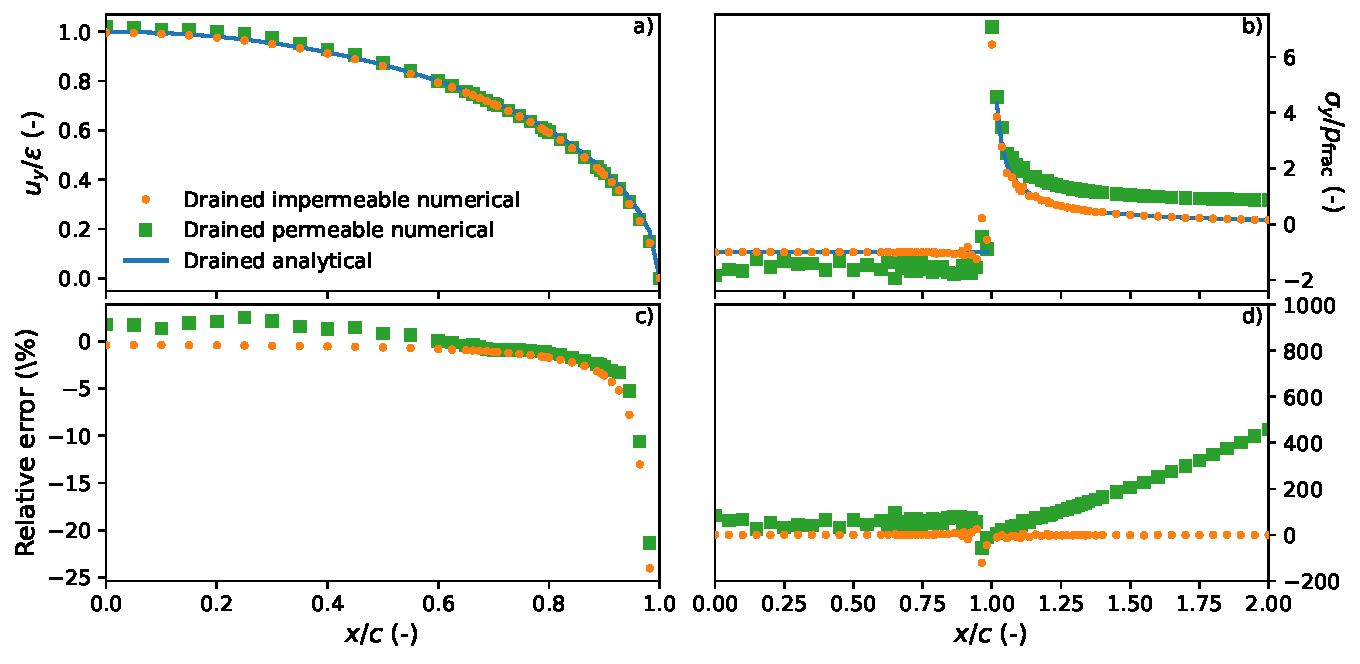
\includegraphics[width=1\textwidth]{../figures/drained}
    \caption{Comparison of the displacements and stress for the drained solution with the analytical solution for the cases of an impermeable and a permeable fracture. \textbf{a)} and \textbf{b)} compares the displacements and stress respectively, while \textbf{c)} and \textbf{d)} shows the relative error of the numerical solutions for the displacement and stress.}
    \label{fig:drained}
\end{figure}
\FloatBarrier

\subsection{Temporal evolution}

The analytical solution can only compute an opening for an undrained and drained case and is detached from any kind of temporal evolution. The numerical solution is then interesting to analyse for this case. Figure \ref{fig:time} shows the behavior of the problem through time for the fracture opening, average pressure in the domain and fluxes at the fracture. The impermeable fracture follows an intuitive path through time, opening monotonically towards the maximum aperture. However, the permeable fracture shows a very interesting, non monotonic behavior. As the fracture initially opens, it then suddenly starts closing before opening back towards the maximum aperture. This difference between the two cases is well shown in the animation \texttt{fracture_opening.gif}. This animation also shows the temporal evolution of the pressure profile at the bottom boundary. The inital punch causes negative pressure at the fracture tip, smoothly resolved as the simulation evolves. The slight increase in pressure at the fracture location in the impermeable case reaches the ambient pressure of zero while the pressure goes to $p_{\text{frac}}$ everywhere in the domain for the permeable case. This behavior is also shown in the animation \texttt{pressure_evolution.gif}. Finally, there is an interesting difference between the fluxes at the fracture location for the impermeable and the permeable case. The impermeable case shows very little fluxes for a small amount of normalized time (barely 10$^{-6}$s). In the permeable case, we initially see negative fluxes at the fracture for the same amount of time as there is flux in the impermeable case, before the fluxes start going into the medium. The cumulative normalized time-integrated fluxes (shown by the dashed lines in figure \ref{fig:time}c) show the total "volume" of fluid that entered the medium.

\begin{figure}[h]
    \centering
    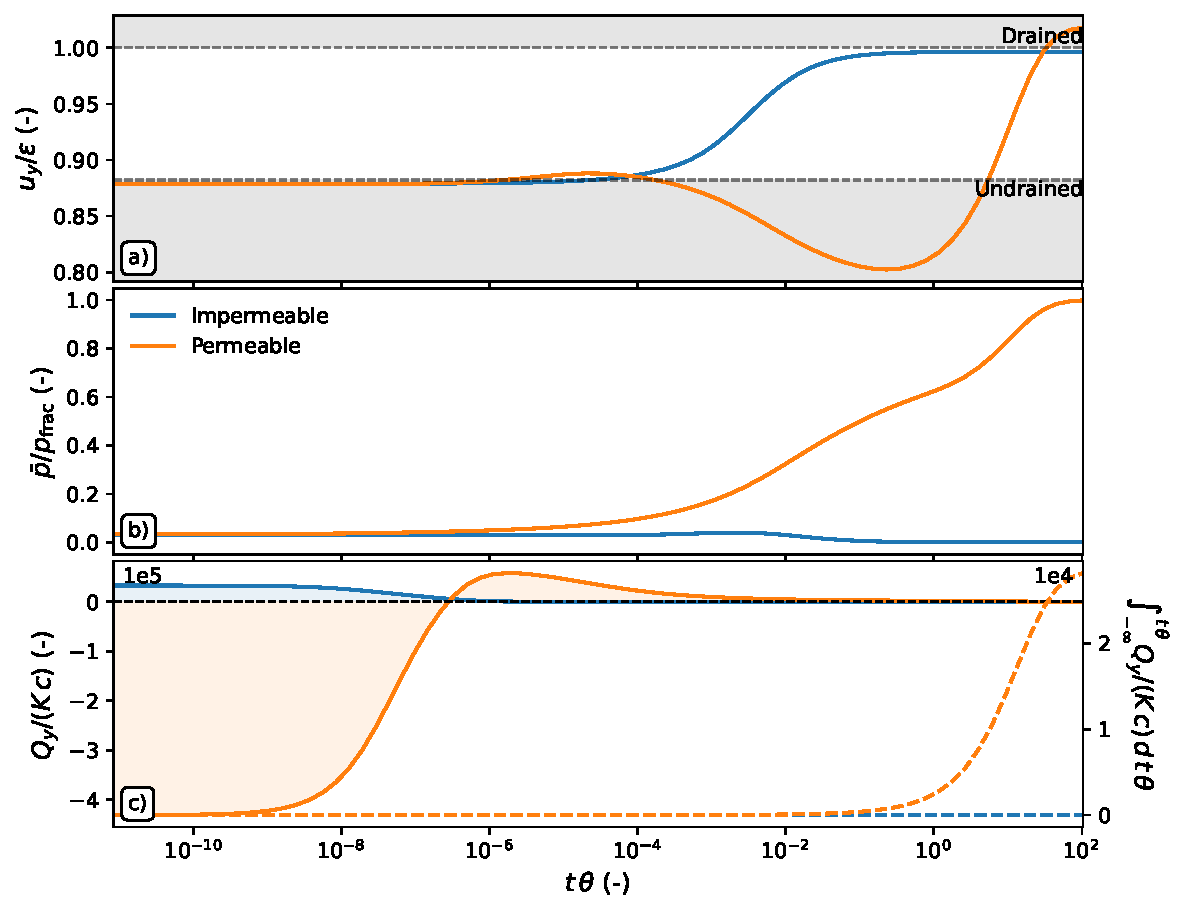
\includegraphics[width=1\textwidth]{../figures/time_behavior}
    \caption{Temporal evolution of the problem. \textbf{a)} shows the opening of the fracture, \textbf{b)} the evolution of the average pressure in the domain and \textbf{c)} shows the fluxes at the fracture.}
    \label{fig:time}
\end{figure}

\FloatBarrier

\section{Discussion}

\subsection{Differences with the analytical solution}
Both the impermeable and the permeable cases show very similar behavior in the undrained and drained cases. The error metric chosen, the relative error, might be a poor exhibit because of the singular values of the displacement and stress at the fracture tip. However, they do a good job in showcasing the similarities between the different solutions everywhere else in the observed domain. The permeable solution is however different in the sense that the effective stress is influenced by the pore pressure. It is interesting to note that previous testing of the numerical solution with linear triangle elements resulted in underestimating the displacements at the fracture; it seems that quadratic elements better approximate the behavior of the problem.

\subsection{Temporal evolution of the fracture}
The differences between the temporal evolution of the fracture in both the impermeable and permeable case is by far the most interesting mechanism in this problem. While the non-monotonic behavior of the permeable fracture can be initially non-intuitive, it can be explained by the pressure difference in the domain. In the undrained case, the initial punch causes a slight increase in pressure, progressively resolved as the deformation is accommodated. However, in the permeable case, we see not only this initial increase in pressure caused by the punch but also a gradual increase in pressure caused by the fixed head at the fracture; the initial pressure difference is so great that the fracture initially closes briefly before reaching again it's maximum aperture as the pressure difference diminishes in the rest of the domain. It is also important to note that this non-monotonic behavior occurs in an extremely short time span, of under 0.01 normalized seconds, while the rest occurs in over 100. 

\subsection{Fluxes at the fracture}
It is interesting to observe negative vertical fluxes at the fracture instantly after the punch. The intuitive mechanism would have been that the fluids would have percolated towards the medium as the pressure difference would have been greater. However, this phenomenon can possibly be caused by the instantaneous loading and the undrained behavior of the medium and or numerical difficulties occurring at very early time. The fluxes however quickly begin to flow inwards the medium, as would be expected of a constant head at the fracture. While there are some inward flux initially in the impermeable case, the time span is so small that virtually no volume of fluid has percolated into the medium at the end of the simulation.

\section{Conclusion}

This report has shown an attempt of a numerical solution for the pressurization of a fracture in a homogeneous medium. While successful in some regards, the results presented are vulnerable of many underlying simplifications, more rigorously described in the previous sections. The most important shortcomings of this work can be synthesized in the two following points:
\begin{itemize}
	\item The opening boundary conditions are unrealistic. In the real world, the pressure wouldn't be the same everywhere; a known imposed flux would be imposed at the borehole. While seemingly simple, this would imply the implementation of a fluid flow law in fractures.
	\item The fracture is of fixed length. While it is an interesting problem to study, it is limiting in it's usefulness to reality. The main application of this work would be to apply to hydraulic fracturation of rocks, in which one would want to cause the propagation of fracture in a medium. This would imply the implementation of much more complex and non-linear behaviors than the present work attempt to show.
\end{itemize}

While vulnerable by those limitations, this work was a great opportunity to study finite element modeling in geomechanics and the coupling between fluid flow in porous media and elasticity.

\bibliographystyle{apacite}
\bibliography{References}

\end{document}
